\documentclass[]{article}
\usepackage{lmodern}
\usepackage{amssymb,amsmath}
\usepackage{ifxetex,ifluatex}
\usepackage{fixltx2e} % provides \textsubscript
\ifnum 0\ifxetex 1\fi\ifluatex 1\fi=0 % if pdftex
  \usepackage[T1]{fontenc}
  \usepackage[utf8]{inputenc}
\else % if luatex or xelatex
  \ifxetex
    \usepackage{mathspec}
  \else
    \usepackage{fontspec}
  \fi
  \defaultfontfeatures{Ligatures=TeX,Scale=MatchLowercase}
\fi
% use upquote if available, for straight quotes in verbatim environments
\IfFileExists{upquote.sty}{\usepackage{upquote}}{}
% use microtype if available
\IfFileExists{microtype.sty}{%
\usepackage{microtype}
\UseMicrotypeSet[protrusion]{basicmath} % disable protrusion for tt fonts
}{}
\usepackage[margin=1in]{geometry}
\usepackage{hyperref}
\hypersetup{unicode=true,
            pdftitle={Using QueryLibrary},
            pdfauthor={Peter Rijnbeek},
            pdfborder={0 0 0},
            breaklinks=true}
\urlstyle{same}  % don't use monospace font for urls
\usepackage{color}
\usepackage{fancyvrb}
\newcommand{\VerbBar}{|}
\newcommand{\VERB}{\Verb[commandchars=\\\{\}]}
\DefineVerbatimEnvironment{Highlighting}{Verbatim}{commandchars=\\\{\}}
% Add ',fontsize=\small' for more characters per line
\usepackage{framed}
\definecolor{shadecolor}{RGB}{248,248,248}
\newenvironment{Shaded}{\begin{snugshade}}{\end{snugshade}}
\newcommand{\AlertTok}[1]{\textcolor[rgb]{0.94,0.16,0.16}{#1}}
\newcommand{\AnnotationTok}[1]{\textcolor[rgb]{0.56,0.35,0.01}{\textbf{\textit{#1}}}}
\newcommand{\AttributeTok}[1]{\textcolor[rgb]{0.77,0.63,0.00}{#1}}
\newcommand{\BaseNTok}[1]{\textcolor[rgb]{0.00,0.00,0.81}{#1}}
\newcommand{\BuiltInTok}[1]{#1}
\newcommand{\CharTok}[1]{\textcolor[rgb]{0.31,0.60,0.02}{#1}}
\newcommand{\CommentTok}[1]{\textcolor[rgb]{0.56,0.35,0.01}{\textit{#1}}}
\newcommand{\CommentVarTok}[1]{\textcolor[rgb]{0.56,0.35,0.01}{\textbf{\textit{#1}}}}
\newcommand{\ConstantTok}[1]{\textcolor[rgb]{0.00,0.00,0.00}{#1}}
\newcommand{\ControlFlowTok}[1]{\textcolor[rgb]{0.13,0.29,0.53}{\textbf{#1}}}
\newcommand{\DataTypeTok}[1]{\textcolor[rgb]{0.13,0.29,0.53}{#1}}
\newcommand{\DecValTok}[1]{\textcolor[rgb]{0.00,0.00,0.81}{#1}}
\newcommand{\DocumentationTok}[1]{\textcolor[rgb]{0.56,0.35,0.01}{\textbf{\textit{#1}}}}
\newcommand{\ErrorTok}[1]{\textcolor[rgb]{0.64,0.00,0.00}{\textbf{#1}}}
\newcommand{\ExtensionTok}[1]{#1}
\newcommand{\FloatTok}[1]{\textcolor[rgb]{0.00,0.00,0.81}{#1}}
\newcommand{\FunctionTok}[1]{\textcolor[rgb]{0.00,0.00,0.00}{#1}}
\newcommand{\ImportTok}[1]{#1}
\newcommand{\InformationTok}[1]{\textcolor[rgb]{0.56,0.35,0.01}{\textbf{\textit{#1}}}}
\newcommand{\KeywordTok}[1]{\textcolor[rgb]{0.13,0.29,0.53}{\textbf{#1}}}
\newcommand{\NormalTok}[1]{#1}
\newcommand{\OperatorTok}[1]{\textcolor[rgb]{0.81,0.36,0.00}{\textbf{#1}}}
\newcommand{\OtherTok}[1]{\textcolor[rgb]{0.56,0.35,0.01}{#1}}
\newcommand{\PreprocessorTok}[1]{\textcolor[rgb]{0.56,0.35,0.01}{\textit{#1}}}
\newcommand{\RegionMarkerTok}[1]{#1}
\newcommand{\SpecialCharTok}[1]{\textcolor[rgb]{0.00,0.00,0.00}{#1}}
\newcommand{\SpecialStringTok}[1]{\textcolor[rgb]{0.31,0.60,0.02}{#1}}
\newcommand{\StringTok}[1]{\textcolor[rgb]{0.31,0.60,0.02}{#1}}
\newcommand{\VariableTok}[1]{\textcolor[rgb]{0.00,0.00,0.00}{#1}}
\newcommand{\VerbatimStringTok}[1]{\textcolor[rgb]{0.31,0.60,0.02}{#1}}
\newcommand{\WarningTok}[1]{\textcolor[rgb]{0.56,0.35,0.01}{\textbf{\textit{#1}}}}
\usepackage{graphicx,grffile}
\makeatletter
\def\maxwidth{\ifdim\Gin@nat@width>\linewidth\linewidth\else\Gin@nat@width\fi}
\def\maxheight{\ifdim\Gin@nat@height>\textheight\textheight\else\Gin@nat@height\fi}
\makeatother
% Scale images if necessary, so that they will not overflow the page
% margins by default, and it is still possible to overwrite the defaults
% using explicit options in \includegraphics[width, height, ...]{}
\setkeys{Gin}{width=\maxwidth,height=\maxheight,keepaspectratio}
\IfFileExists{parskip.sty}{%
\usepackage{parskip}
}{% else
\setlength{\parindent}{0pt}
\setlength{\parskip}{6pt plus 2pt minus 1pt}
}
\setlength{\emergencystretch}{3em}  % prevent overfull lines
\providecommand{\tightlist}{%
  \setlength{\itemsep}{0pt}\setlength{\parskip}{0pt}}
\setcounter{secnumdepth}{5}
% Redefines (sub)paragraphs to behave more like sections
\ifx\paragraph\undefined\else
\let\oldparagraph\paragraph
\renewcommand{\paragraph}[1]{\oldparagraph{#1}\mbox{}}
\fi
\ifx\subparagraph\undefined\else
\let\oldsubparagraph\subparagraph
\renewcommand{\subparagraph}[1]{\oldsubparagraph{#1}\mbox{}}
\fi

%%% Use protect on footnotes to avoid problems with footnotes in titles
\let\rmarkdownfootnote\footnote%
\def\footnote{\protect\rmarkdownfootnote}

%%% Change title format to be more compact
\usepackage{titling}

% Create subtitle command for use in maketitle
\newcommand{\subtitle}[1]{
  \posttitle{
    \begin{center}\large#1\end{center}
    }
}

\setlength{\droptitle}{-2em}

  \title{Using QueryLibrary}
    \pretitle{\vspace{\droptitle}\centering\huge}
  \posttitle{\par}
    \author{Peter Rijnbeek}
    \preauthor{\centering\large\emph}
  \postauthor{\par}
      \predate{\centering\large\emph}
  \postdate{\par}
    \date{2019-08-07}


\begin{document}
\maketitle

{
\setcounter{tocdepth}{2}
\tableofcontents
}
\hypertarget{introduction}{%
\section{Introduction}\label{introduction}}

The QueryLibrary R-package is a repository of OMOP-CDM queries created
and validated by the OHDSI community. The purpose of the library is to
help new users to learn how to query the CDM. The query library can be
used for training purposes, but will also be a valuable resource for the
more experienced users. The tool utomatically renders the queries to the
dialect, cdm and vocabulary schemas as specified in the configuation
settings. Furthermore, it can execute the query against a user's
database.

In this vignette we first explain how to install the tool and then
demonstrate its use.

\hypertarget{installation}{%
\section{Installation}\label{installation}}

Running the package requires R with the package rJava installed. Also
requires Java 1.6 or higher and you need to have the following
dependencies installed in R:

\begin{itemize}
\tightlist
\item
  SQLRender
\item
  DatabaseConnector
\item
  Shiny
\end{itemize}

To install the latest development version, install from GitHub:

\begin{Shaded}
\begin{Highlighting}[]
\KeywordTok{install.packages}\NormalTok{(}\StringTok{"devtools"}\NormalTok{)}
\NormalTok{devtools}\OperatorTok{::}\KeywordTok{install_github}\NormalTok{(}\StringTok{"ohdsi/QueryLibrary"}\NormalTok{)}
\end{Highlighting}
\end{Shaded}

Once installed, you can try out the Shiny app that comes with the
package:

\begin{Shaded}
\begin{Highlighting}[]
\KeywordTok{library}\NormalTok{(QueryLibrary)}
\KeywordTok{launchQueryLibrary}\NormalTok{()}
\end{Highlighting}
\end{Shaded}

\begin{figure}
\centering
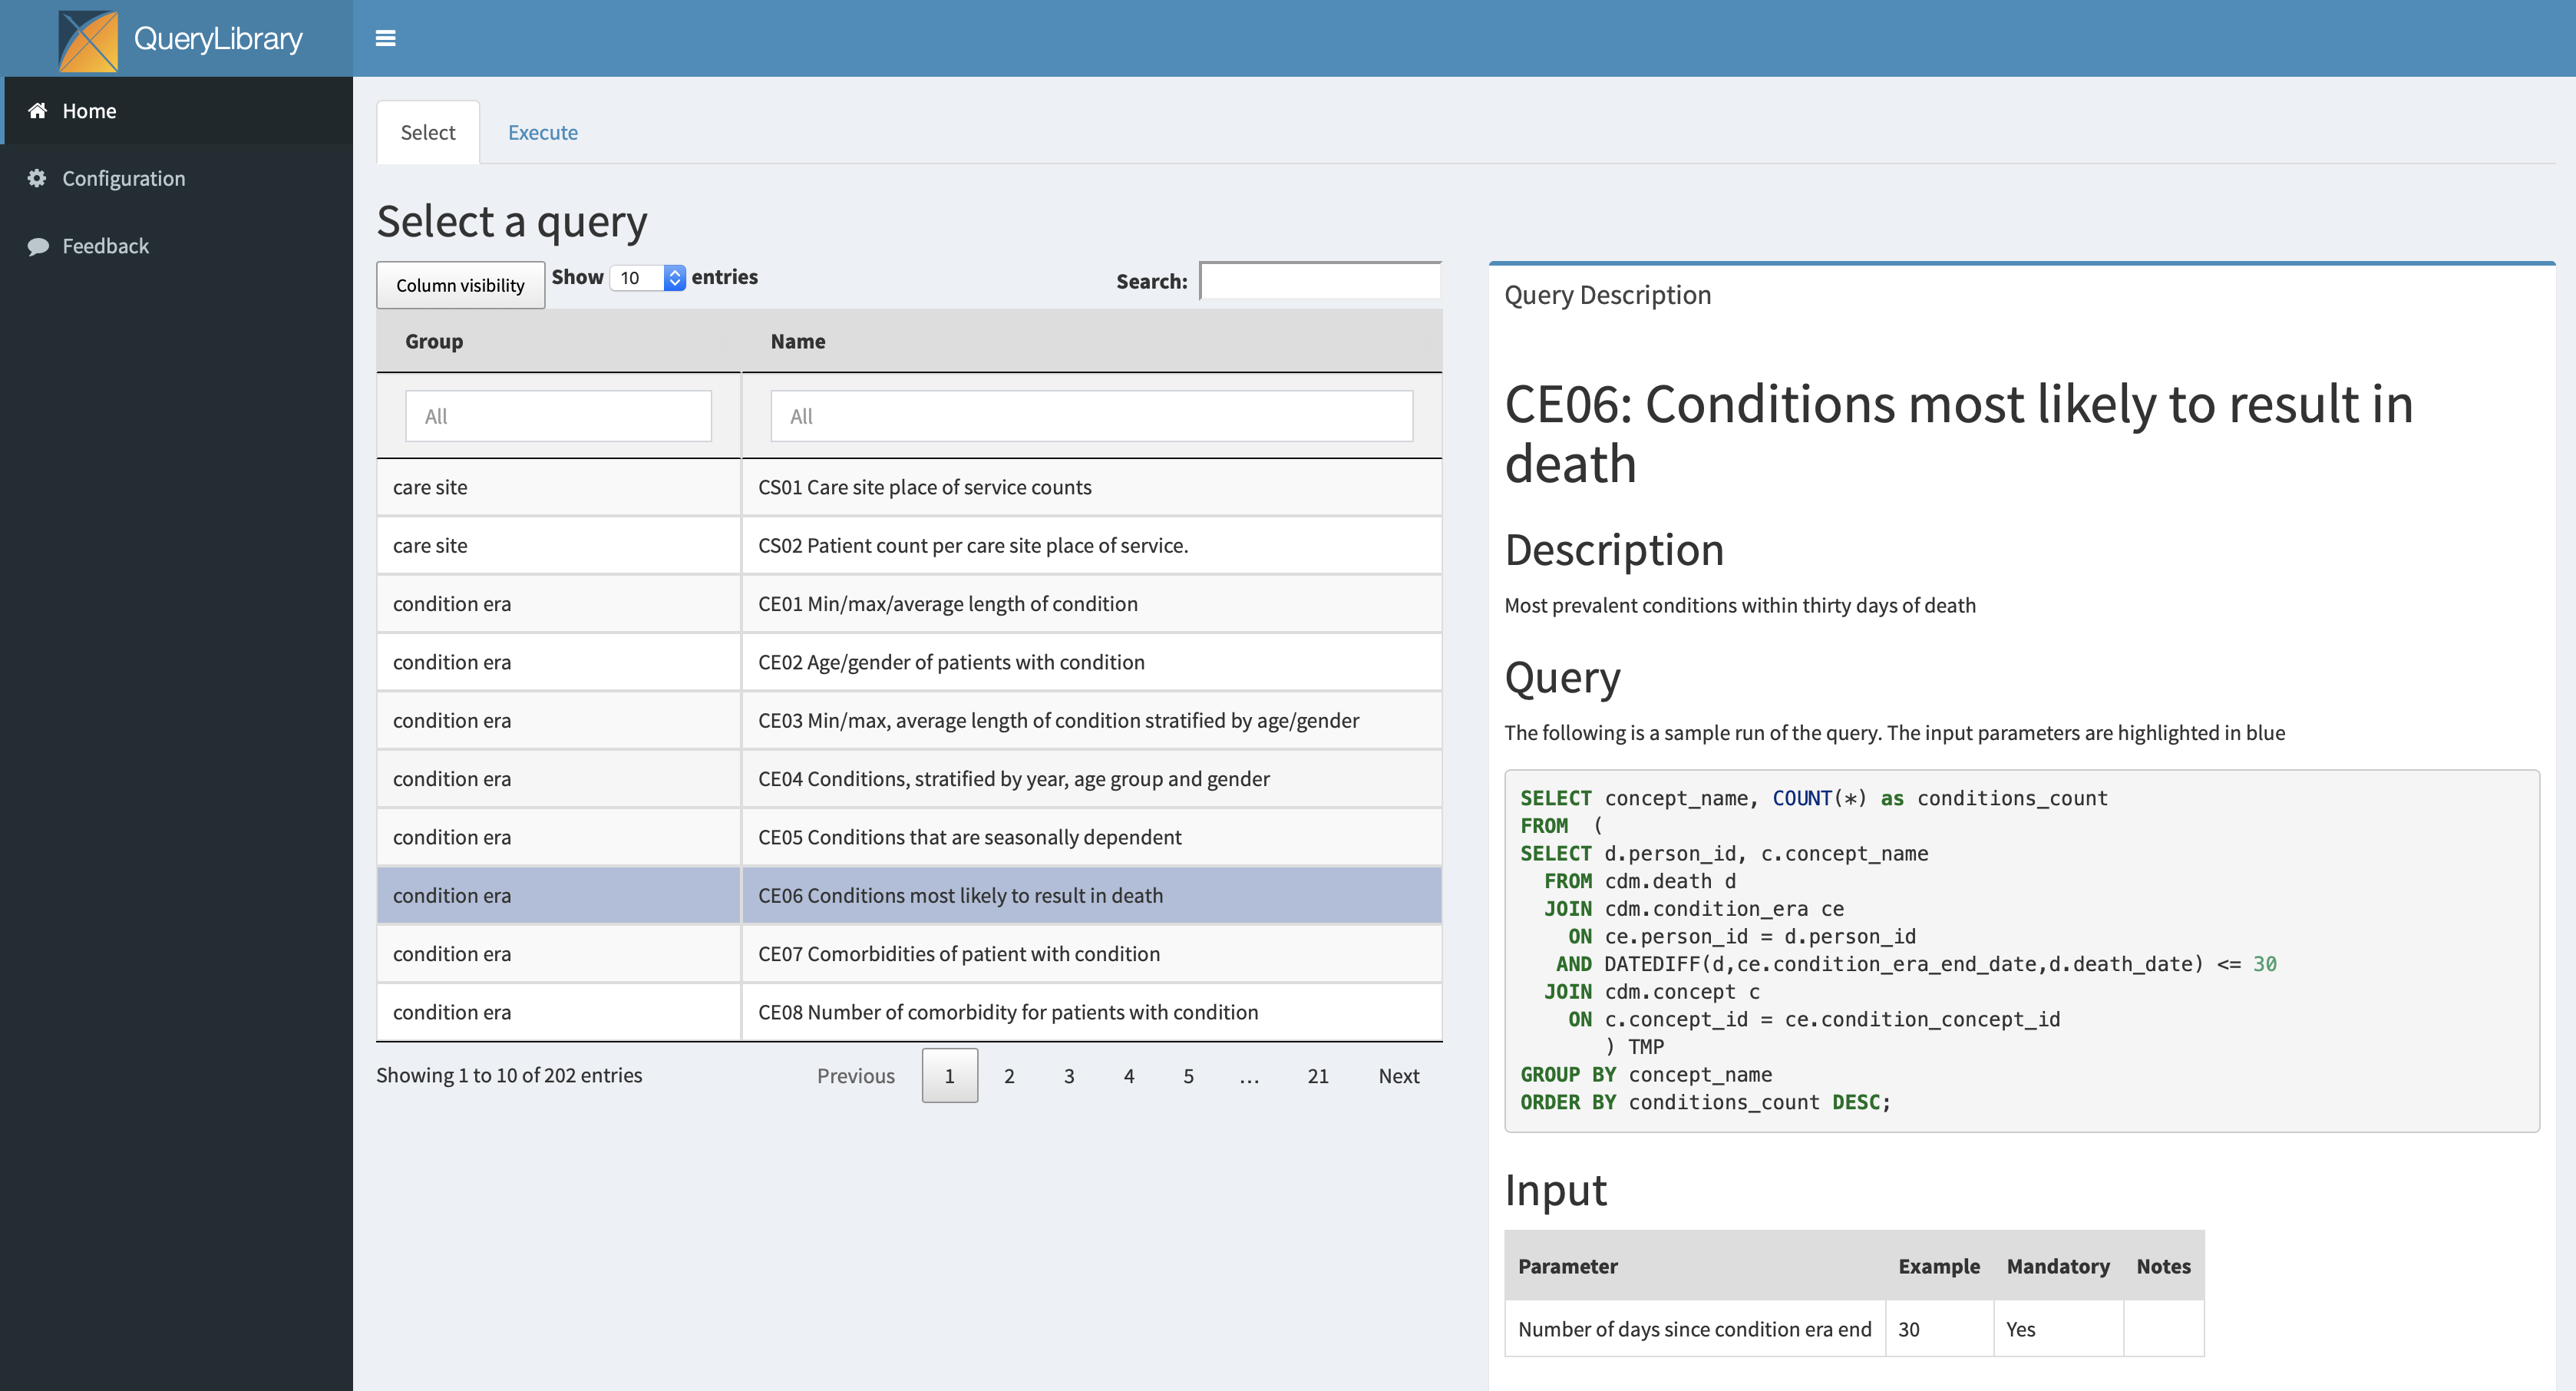
\includegraphics{home.png}
\caption{QueryLibrary home page}
\end{figure}

\hypertarget{configuration-settings}{%
\section{Configuration settings}\label{configuration-settings}}

First, you have to fill in the configuration settings by clicking on
configuration in the menu.

\begin{figure}
\centering
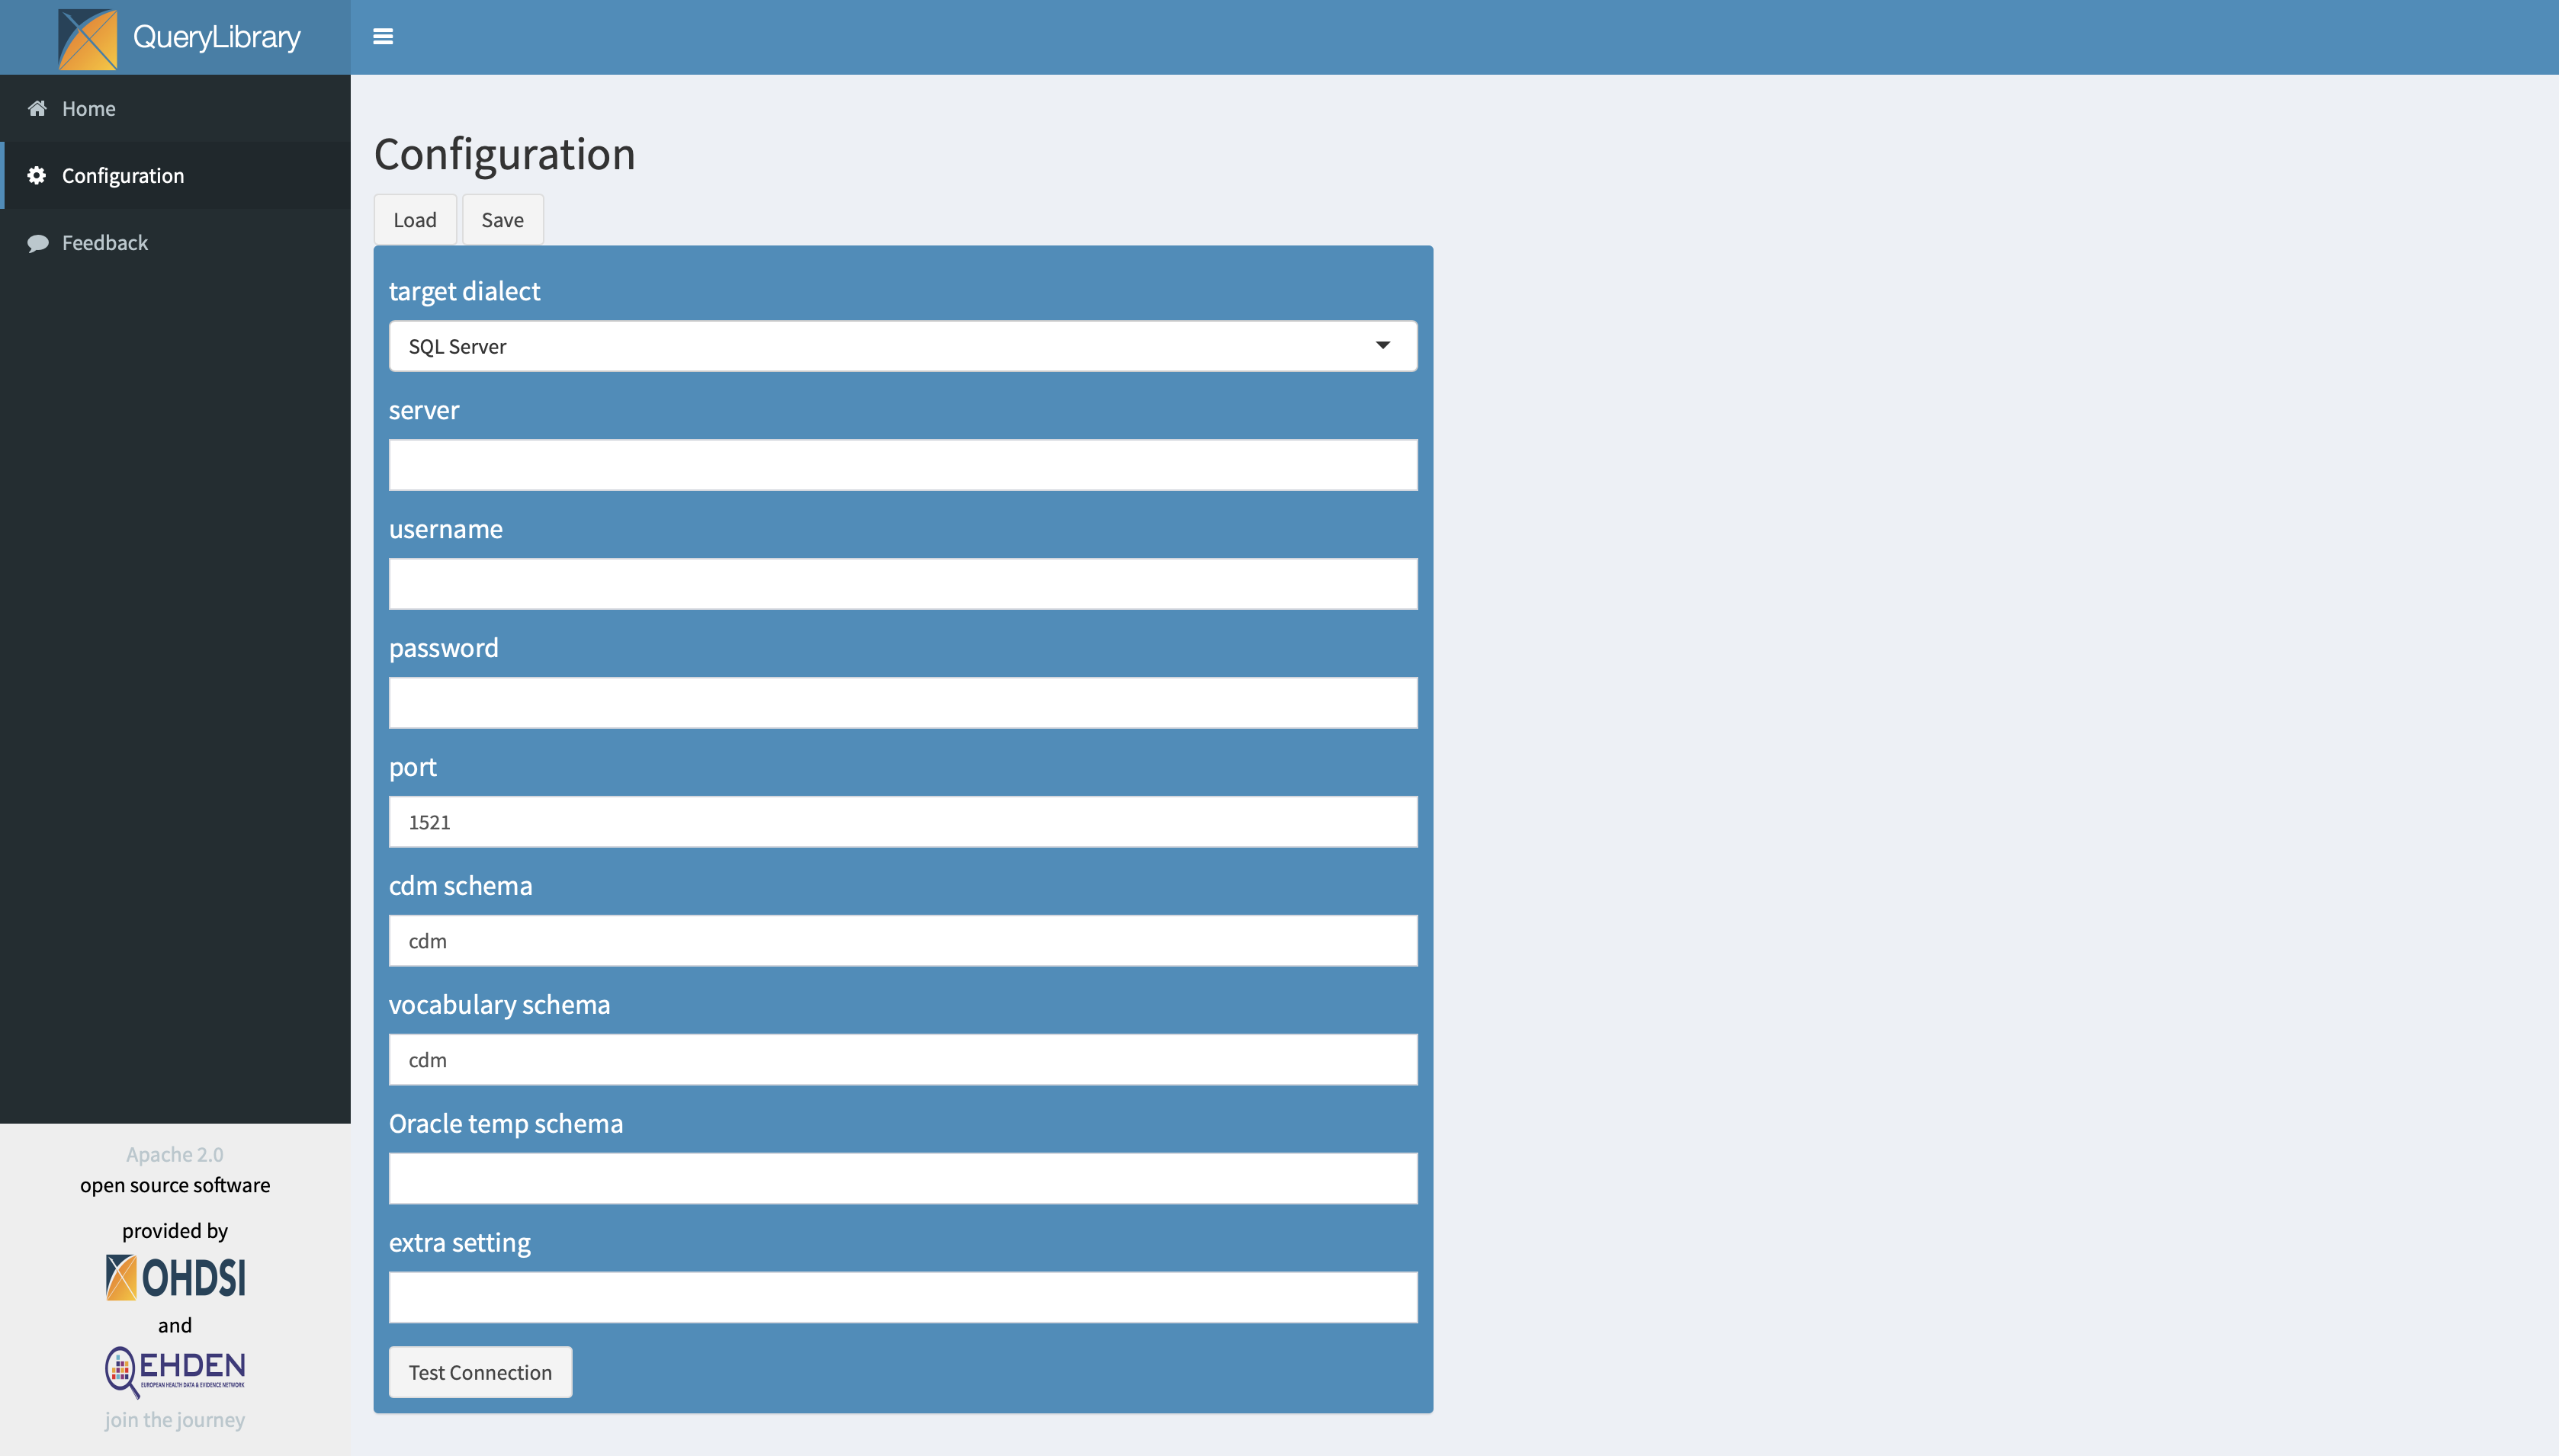
\includegraphics{config.png}
\caption{Configuration page}
\end{figure}

The configuration section allows the user to set the dialect and other
connection details for the CDM. This settings file can be saved and
loaded using the buttons on the top of the page. The cdm and vocabulary
schema will be filled in automatically in parameretised queries.

\hypertarget{selecting-and-running-a-query}{%
\section{Selecting and running a
query}\label{selecting-and-running-a-query}}

Using the library table the user can select a query. The markdown file
of the query can be see on the right. The Execute tab allows the user to
import the selected query, edit the query (the window can be made bigger
if needed), run, copy, and save the query. The tool will show a counter
when the query is running and will show the results table below the
query.

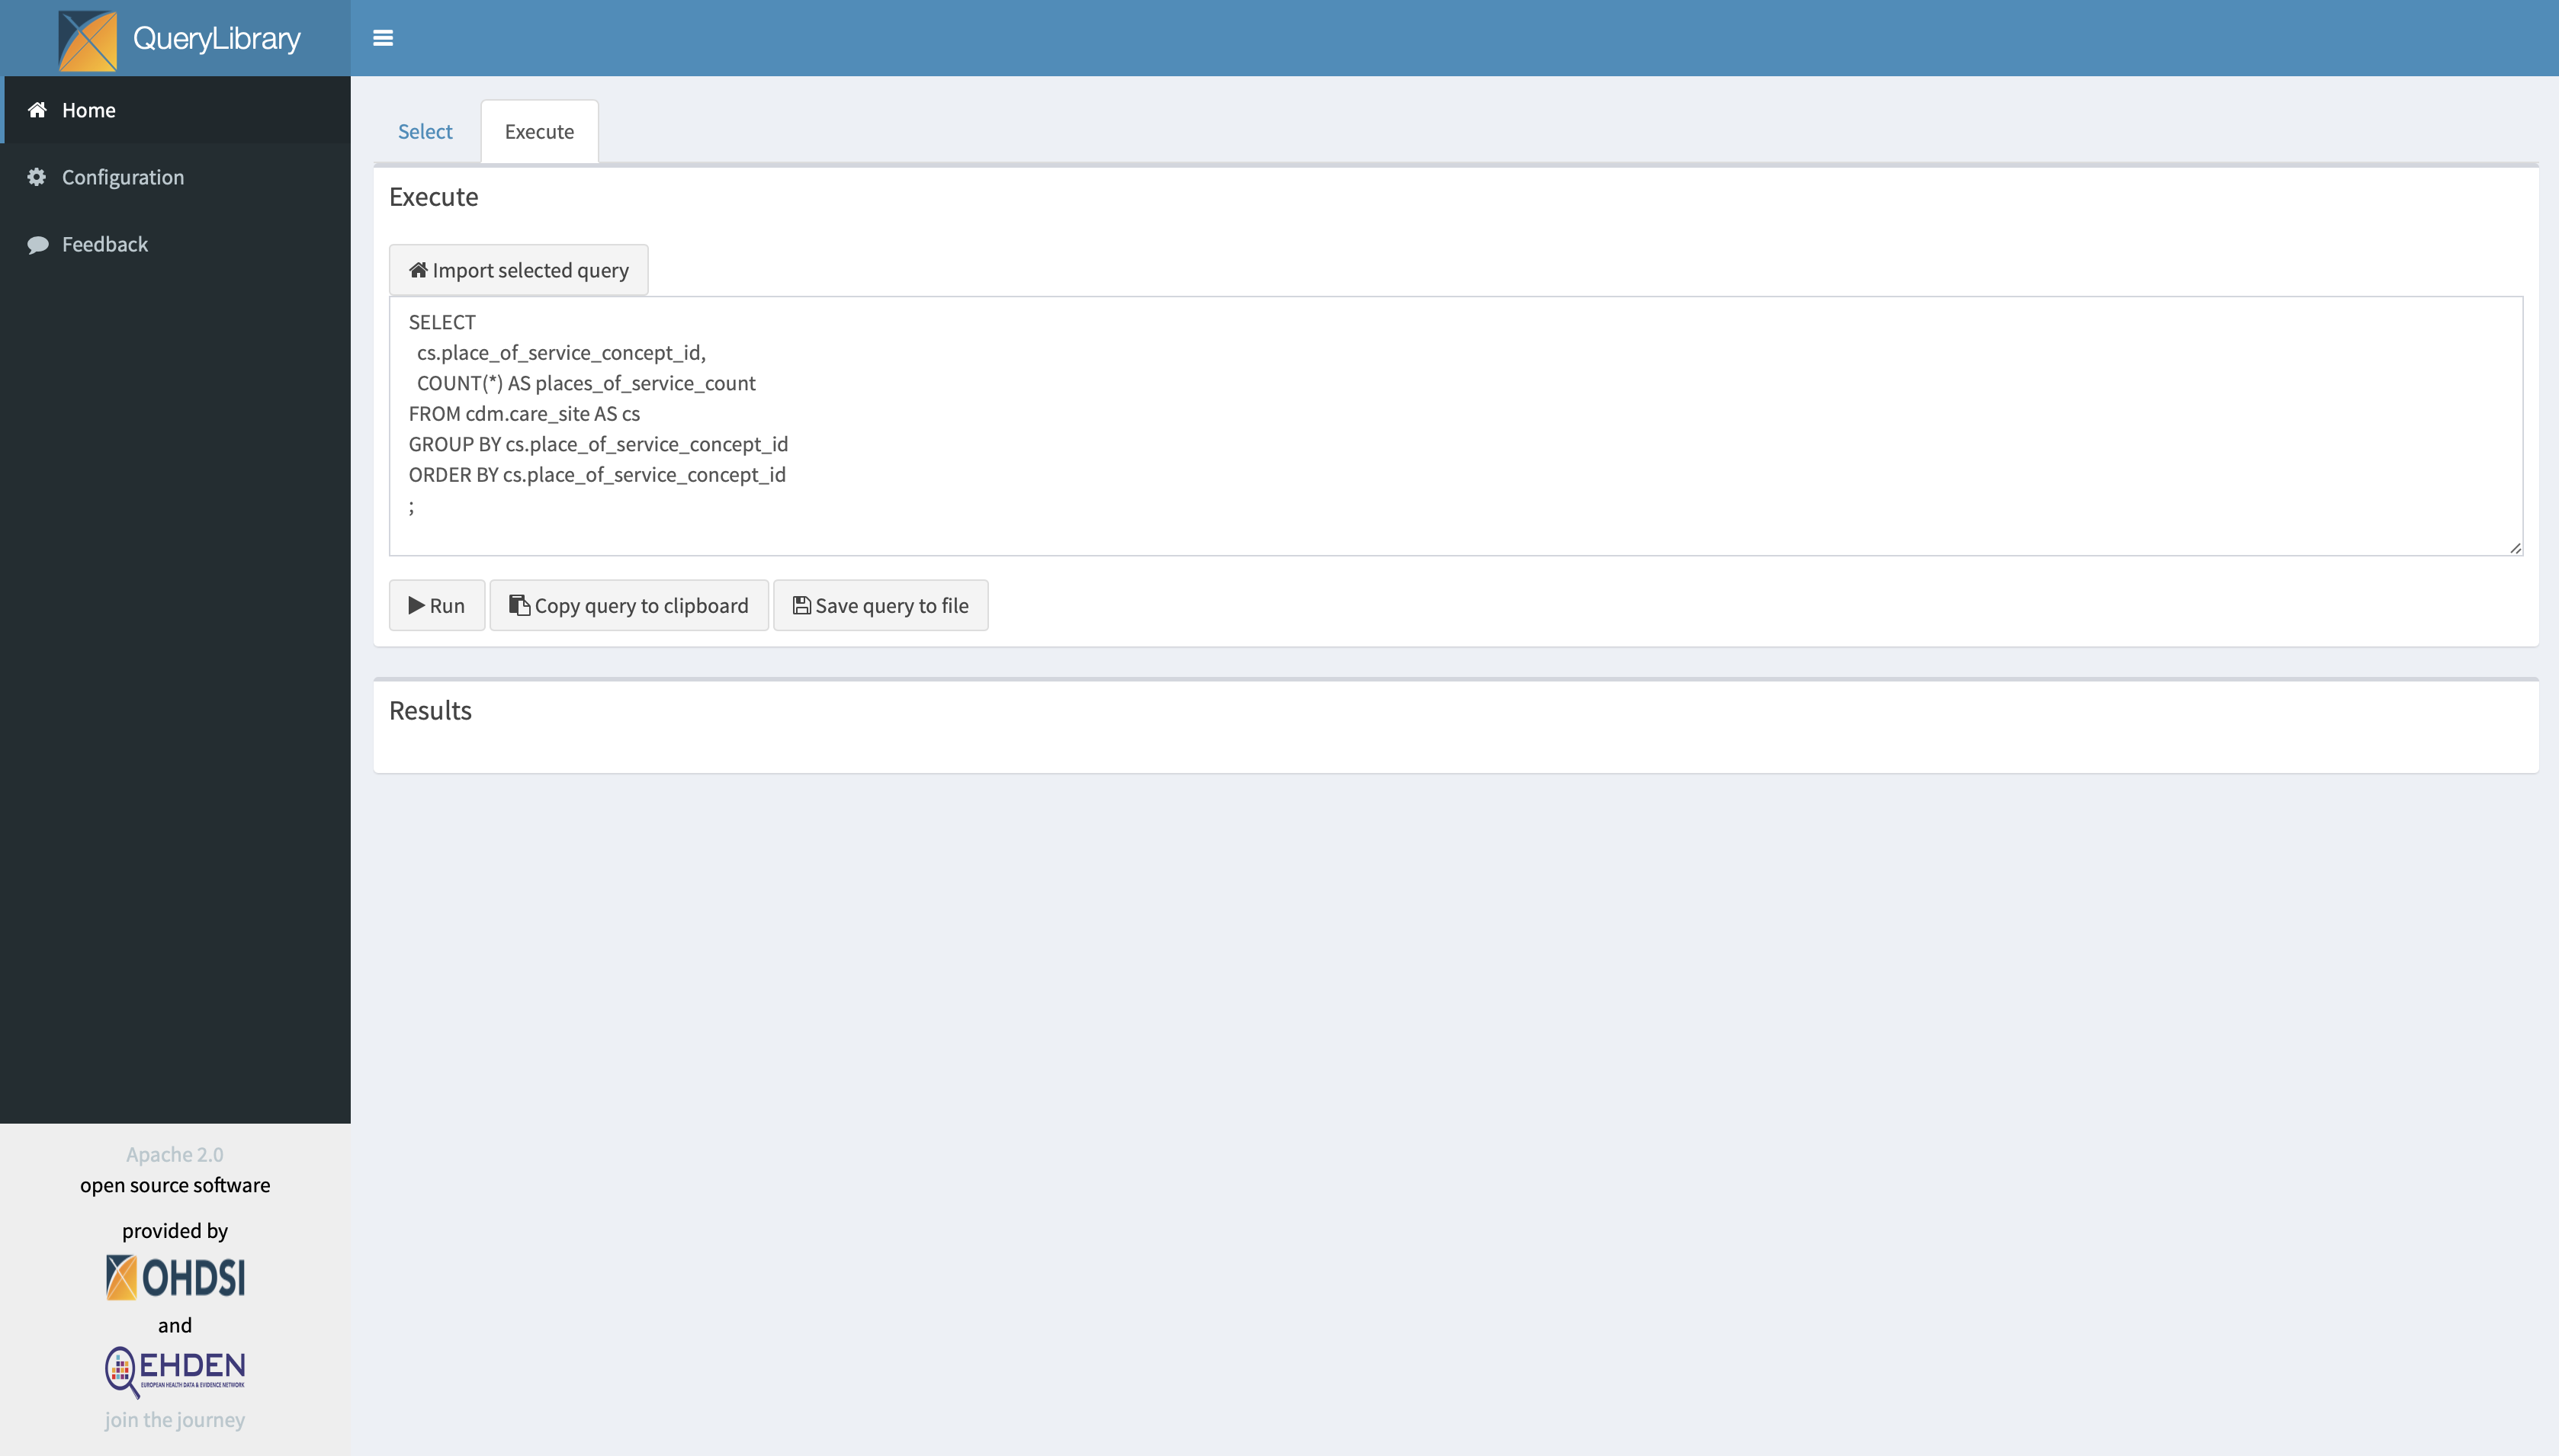
\includegraphics{execute.png} The path to the queries folder can be set
in the global.R file. Here you can also set the default settings name
and specify if you allow the executing of queries:

\begin{Shaded}
\begin{Highlighting}[]
\NormalTok{queryFolder =}\StringTok{ "./queries"}
\NormalTok{configFilename =}\StringTok{ "settings.Rds"}
\NormalTok{allow_execute =}\StringTok{ }\OtherTok{TRUE}
\end{Highlighting}
\end{Shaded}

We added the allow\_execute option since you may not want users to load
and save settings files to the server or like to connect to databases
when you install the Shiny Application on a public sever like
data.ohdsi.org

\hypertarget{extending-the-library}{%
\section{Extending the library}\label{extending-the-library}}

We would like to increase the number of queries in the library and like
the community to drive this. If there are suggestions please post them
in the issue tracker or even better do a pull request and we will review
and approve your query.

To extend the library you can add a new Markdown file in the queries
folder. The query file contains a description of the query, and explains
the input variables, output table, and provides an output example. The
following information is parsed from the markdown files using tags:

\begin{itemize}
\tightlist
\item
  Group. Allows to group queries, e.g.~by domain
\item
  Name. The name of the query in the search table.
\item
  CDM-Version. The version this query runs on, e.g. \textgreater{}5.0
\item
  Author. The person responsible for writing the query
\item
  Query. The query is taken from the .Md file, rendered using SqlRender
  and is shown to the user in its preferred dialect. You should add
  @vocab or @cdm as parameters in the query if you refer to the cdm of
  vocab schema.
\end{itemize}

Note that if you add queries you have to follow the (OHDSI code style
for
SQL){[}\url{https://www.ohdsi.org/web/wiki/doku.php?id=development:ohdsi_code_style_for_sql}{]}.

We have added functionality to test all the queries against multiple
database management systems (see extra/Test.R). This will be executed on
your new query before we approve it.

\hypertarget{references}{%
\section{References}\label{references}}

\begin{itemize}
\tightlist
\item
  Vignette:
  \href{https://github.com/OHDSI/QueryLibrary/blob/master/inst/doc/UsingQueryLibrary.pdf}{Using
  QueryLibrary}
\item
  Package manual:
  \href{https://github.com/OHDSI/QueryLibrary/blob/master/extras/QueryLibrary.pdf}{QueryLibrary
  manual}
\item
  Developer questions/comments/feedback: OHDSI Forum
\item
  We use the GitHub issue tracker for all bugs/issues/enhancements
\end{itemize}

\hypertarget{acknowledgement}{%
\section{Acknowledgement}\label{acknowledgement}}

This work was performed within the European Health Data \& Evidence
Network (\href{https://www.ehden.eu}{EHDEN}) project in collaboration
with OHDSI. The European Health Data \& Evidence Network has received
funding from the Innovative Medicines Initiative 2 Joint Undertaking
(JU) under grant agreement No 806968. The JU receives support from the
European Union's Horizon 2020 research and innovation programme and
EFPIA.


\end{document}
